%
% File          : 5GAKA-proof.tex
% Description   : 5G-AKA Proof Paper
% Authors       : Clayton & Harmon
%
% Last Modified : Fri Dec  1 08:17:28 EST 2000
%
% BDOC PARAM offset=0in,0in

% Page style
\documentclass[11pt, pdftex]{article}
\usepackage{epsf}
\usepackage{epsfig}
\usepackage{times}
\usepackage{ifthen}
\usepackage{comment}

\usepackage[margin=1in]{geometry}


\title{5G-AKA: A Formal Verification}
\author{David Clayton and Ira Harmon}
\date{November 29, 2018}


\begin{document}
\maketitle
\textbf{Abstract:} 
The 5th generation of cell phone technology is scheduled to be deployed by 2021.  It will connect more people around the world than any prior generation.  The 5G protocol suite includes modifications of existing protocols as well as new protocols.  However, the foundation of 5G security rest upon the 5G-AKA protocol.  Since inception, 5G-AKA has gone through multiple revisions due to discovered vulnerabilities.  In this paper the most recent version of the protocol is tested through symbolic analysis and recommendations are made that would improve its overall security.

\newpage
\section{Introduction}
By 2019 over 5 Billion people are expected to own a mobile phone.  Currently over 62 percent of the world population uses mobile phones.  As cell phones become more pervasive their use touches every aspect of modern life: Facebook updates, news, and banking transactions are all increasingly done via cell.  At this critical time in the evolution of cellular technology, 3GPP, the body that standardizes cell phone protocols is preparing to deploy 5G.  And while 5G promises to connect more users with better service than previous generations, the unrestrained growth of the technology makes the security implications of 5G critical.  5G-AKA (Authentication and Key Agreement) is the first line of defense in securing mobile communications.  The protocol authenticates the user and distributes long term keys.  The most recent version of the protocol is outlined in 3GPP Publication TS 33.501 V15.2.0.  In this paper we validate the most recent version of the protocol through symbolic analysis.  

\section{The 5G-AKA Protocol}

5G-AKA is similar to authentication protocols used in previous generations.  5G allows for authentication via 5G-AKA or EAP-AKA.  For the purposes of this paper, the focus is 5G-AKA.  There are at least 4 actors in the 5G authentication process.  

\begin{quote}
1) \textbf{UE} (user equipment) -  The UE is a mobile device.  It is identified by its SUPI (SUbscription Permanent   
Identifier).  The SUPI serves the same purpose as the IMSI in previous generations.

2) \textbf{SEAF} (SEcurity Anchor Function) - The SEAF is co-located with the AMF (core Access Management Function).  The SEAF creates a key, $K_{seaf}$, that is used to encrypt all communications during authentication  \cite{zhang2017overview}.  This key is also used to derive the session key post authentication.  The SEAF communicates with the UE via the SUCI (SUbscriper Concealed Identifier).  This equivalent to the TMSI in previous generations. 

3) \textbf{AUSF} (AUthentication Server Function) -  The AUSF handles authentication requests for the 3GPP network and non-3GPP network.  It informs the UDM of successful and failed authentications.  

4) \textbf{UDM} (Unified Data Management) - The ARPF (Authentication credential Repository and Processing Function) is co-located with the UDM. The ARPF is located in the home network of the UE. The ARPF stores the long term key of the UE.  This is the same key stored on the SIM card of the UE.  The ARPF also stores the SUPI associated with each SUCI.  It communicates an authentication vector back to the AUSF after receiving an authentication request.  Because of its credential store it is the most secured component in the network \cite{cremers2017comprehensive}.

\end{quote}

\graphicspath{ {./images/} }
\begin{figure}[h]
	\begin{center}
		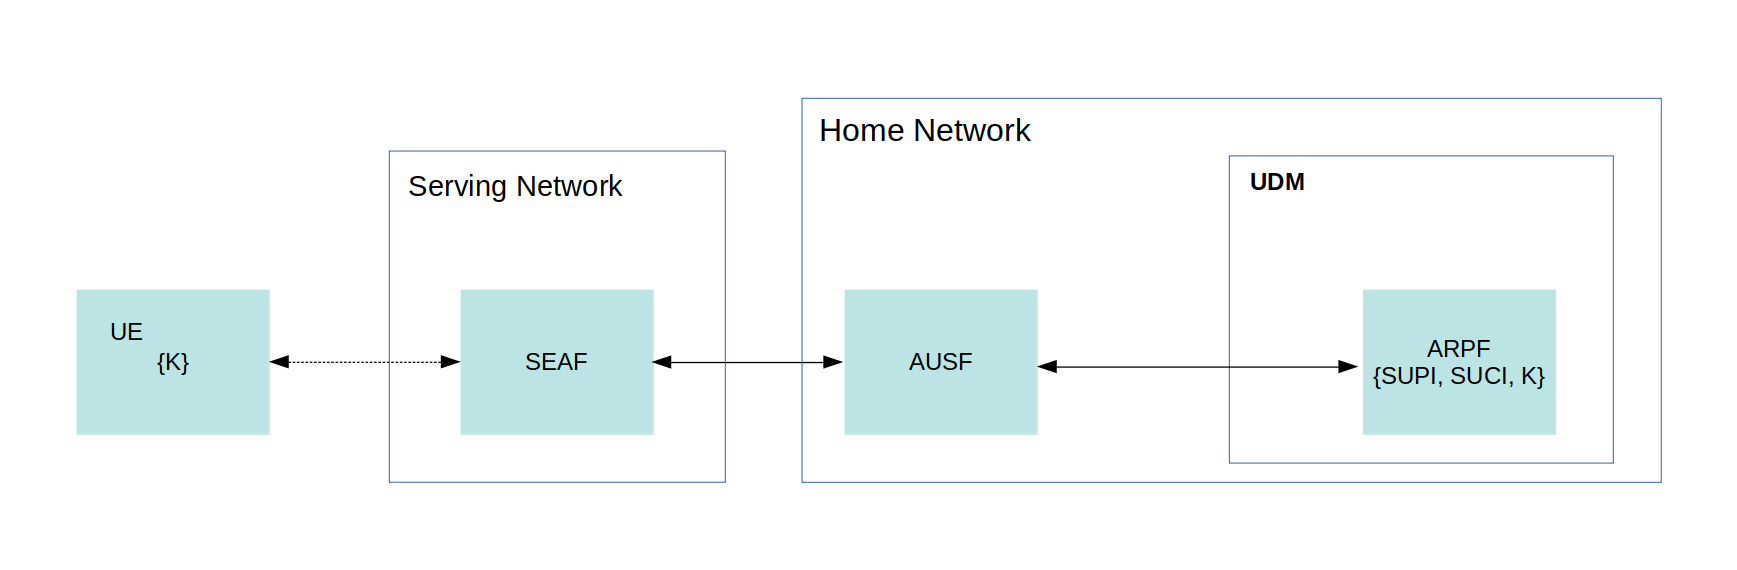
\includegraphics[scale=0.21]{Figure2_1.png}
	\end{center}
	\caption{Dashed lines indicate insecure connections.}
\end{figure}

Figure 2.1 gives a high level overview of the connections between the four components.

The protocol begins with an authorization request.  The request can be initiated by the UE or the SEAF.  


















\section{Related Work}
The Tamarin-Prover is software for the symbolic analysis and verification of security protocols.



     
\nocite{*}
\bibliography{References}
\bibliographystyle{plain}
\end{document}
